

\documentclass{article}
\usepackage[latin1]{inputenc}
\usepackage[ngerman]{babel}
\usepackage{setspace}
\usepackage{amssymb}
\usepackage{amsmath}
\usepackage{hyperref}
\usepackage{graphicx}
\usepackage{rotating}
\usepackage{textcomp}
\begin{document}

These are our first tries to fit ERGM-models. First approach: Try to fit a model suggested for starting by Robins and Lusher (2011). Model does degenerate quickly. Thus we try to find statistics which are responsible for degeneration by extracting each term in a seperate model and check the perfomance via mcmc.diagnostics. This is repeated for every year in our data set (1992 - 2011).
\begin{table}[h]
	\centering
	\caption{ERGM-Terms suggested by Robins and Lusher and the result of their mcmc.diagnostics}
		\begin{tabular}{l|l}
		
		\hline
		ergm-term 											& mcmc.diagnostics 								\\
		\hline
		edges														& converges												\\
		mutual													& converges												\\
		gwidegree(decay, fixed = TRUE)	& works only with decay near one	\\
		gwodegree(decay, fixed = TRUE) 	& degenerates											\\
		gwdsp(fixed = TRUE)							& works, long computation time		\\
		gwesp(fixed = TRUE)							& works, long computation time		\\
		ctriple													& degenerates											\\
		
		\hline
						
		\end{tabular}
	
	\label{tab:stats.robins}
\end{table}

Now we try to find some terms which can replace the terms wich are degenerating or have a long computational time. The idea is to combine all terms which are working fine in new model.


\begin{table}[h]
	\centering
	\caption{Replacement for ERGM-Terms}
		\begin{tabular}{l|l}
		
		\hline
		ergm-term 											& mcmc.diagnostics	 								\\
		\hline
		ostar(2)												& degenerates											 	\\
		dsp(1)													& converges in most years 					\\
		esp(1)													& converges in most years	  				\\
	
		\hline
						
		\end{tabular}
	
	\label{tab:stats.replace}
\end{table}

\begin{itemize}
\item Combining statistics leads to long computing time
\item Thats why we try to estimate parameters for single statistics 
\item Estimation of four different models:
 	\begin{itemize}
	\item edge + mutual,
	\item edge + gwindegree(decay = 0.9, fixed = T),
	\item edge + esp(1),
	\item edge + dsp(1)
	\end{itemize}
\item Time Series of Parameters:
\end {itemize}
\vspace{2.5cm}

\begin{figure}[h]
	\centering
		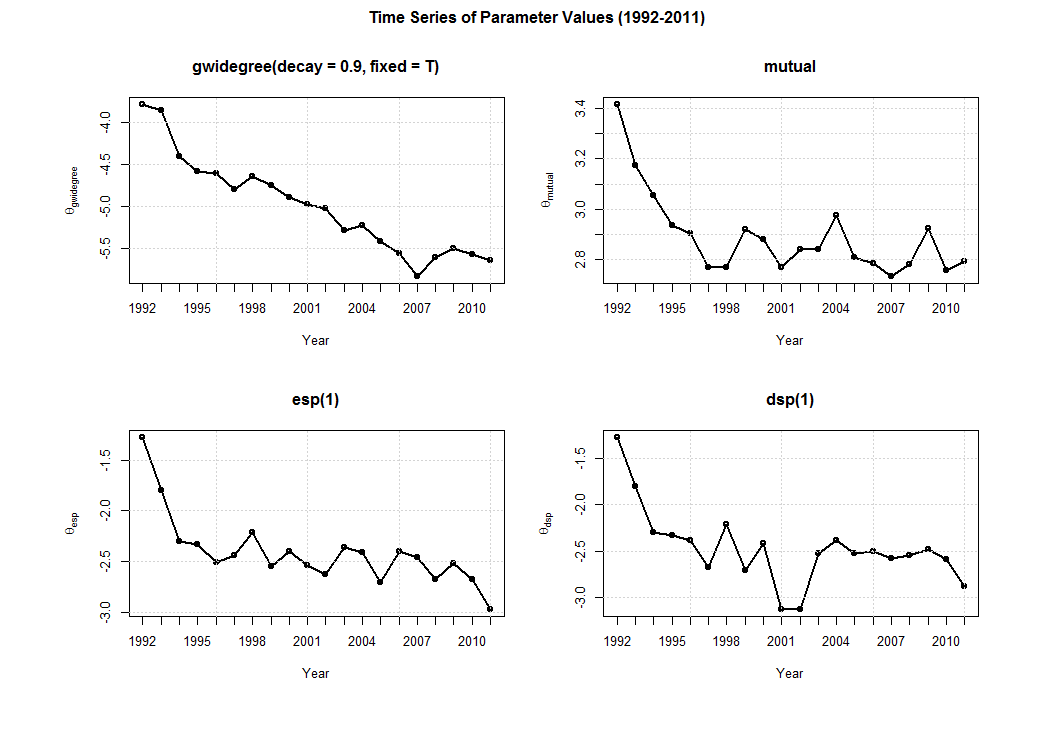
\includegraphics[width=1.30\textwidth, angle = 90]{C:/Users/s10370952/Documents/Consulting/Grafiken/ts_ERGM_coef.png}
	\label{fig:ts_ERGM_coef}
\end{figure}


Interpretation of Time Series:
\begin{itemize}
	\item mutual : Positive value suggests that reciprocated ties are likely. Strength of effect weakens between 1991-1997, then stays quite constant. In our context this means that the weapon trade tends to be symmetric.
	\item gwindegree: Negative popularity spread parameter indicates that most actors have simular levels of popularity (the network is not centralized on in-degree). Strength of effect increases over time. In our context this means that the weapon trade network does not tend to have central importeurs. 
	\item esp(1): A negative effect indicates a low degree of clustering. Strength of effect increases until 1996, then stays quite constant. In our context this means that that the weapon trade network does not tend to form small groups.
	\item dsp(1): This parameter relates to the 2-paths in the networks. A negative estimate indicates that 2-paths tend to be closed (triangles are formed). In our context this means that the weapon trade network tends to form triangles (small groups). This contradicts the findings of the interpretation of esp(1). A joint modeling of both parameters could possibly solve this problem?
	
\end{itemize}

\end{document}